% Indicate the main file. Must go at the beginning of the file.
% !TEX root = ../main.tex

%----------------------------------------------------------------------------------------
% CHAPTER TEMPLATE
%----------------------------------------------------------------------------------------


\chapter{Resultate} % Main chapter title

\label{Chapter4} % Change X to a consecutive number; for referencing this chapter elsewhere, use \ref{ChapterX}

%----------------------------------------------------------------------------------------
% SECTION 1
%----------------------------------------------------------------------------------------
Für die ersten Experimente wurden die Repositories der Racetrack-Projekte ausgewertet. Wie im Kapitel \secref{sec:Projektmodule} erwähnt, findet dieses Projekt im Kontext des Projektmoduls 2 als erstes Projekt statt. Dieses dauert ungefähr vier Wochen, wobei die genaue Anzahl der Tage pro Klasse variieren kann. Das Grundgerüst des Sourcecodes wird in der Aufgabenstellung mitgeliefert, was die Vergleichbarkeit der Projekte erhöht. Ausserdem haben die Studenten schon Erfahrung mit der Handhabung von PullRequests. 

\section{Ergebnisse Racetrack}
Die ersten Analysen zeigen, dass pro Repository durchschnittlich 34.3 PRs erstellt werden. Die Vollzeitklassen erfassen mit durchschnittlich 39.5 PRs pro Projekt mehr PRs als die Teilzeitklassen, die im Schnitt 31.8 erzeugen. Der Median liegt bei 34 PRs.

Bezüglich des Churns weisen die PRs der Racetrack Repos 278.2 geänderte Zeilen auf, wobei der Median bei 94 Zeilen liegt. Die Vollzeitklassen verfügen mit 301.3 über grössere PRs als die Teilzeitklassen mit 260.3 Zeilen. Auch beim Median zeigt sich ein leichter Unterschied: 97 geänderte Zeilen bei den Vollzeit- gegenüber 93 bei den Teilzeitklassen. 

Die durchschnittliche PR-Latenz beträgt insgesamt rund 18 Stunden und 34 Minuten. Die durchschnittliche Latenz in den Teilzeitklassen liegt bei knapp 19 Stunden und 53 Minuten, in den Vollzeitklassen bei etwa 16 Stunden und 53 Minuten. Der Median der Latenzzeit fällt jedoch deutlich kürzer aus und beträgt insgesamt nur rund 37 Minuten. Interessanterweise zeigen die Teilzeitklassen mit einem Median von 28 Minuten eine schnellere Reaktionszeit als die Vollzeitklassen, deren Median bei 48 Minuten liegt.

Auch die Struktur der PRs unterscheidet sich leicht zwischen den Unterrichtsmodellen: Die durchschnittliche Anzahl bearbeiteter Dateien pro PR liegt insgesamt bei 5.66 Dateien. Teilzeitklassen weisen mit 5.85 im Schnitt mehr betroffene Dateien auf als Vollzeitklassen mit 5.42 Dateien. Ebenso zeigt sich bei der durchschnittlichen Anzahl Commits pro PR ein Unterschied: Insgesamt liegt der Durchschnitt bei 7.03 Commits pro PR, wobei Teilzeitklassen auf 6.50 und Vollzeitklassen auf 7.70 Commits pro PR kommen.

\section{Ergebnisse Latency vs. Churn}
Die verschiedenen Farben in der  \autoref{fig:pr-latency-vs-churn-allgemein}  repräsentieren die einzelnen Projekte der Projektgruppen.
Wie in der Abbildung ersichtlich, zeigt sich ein Cluster von Datenpunkten in der linken unteren Ecke. Dabei konzentrieren sich die Punkte vorallem bei einem Churn von unter 1000 Zeilen und unter 100 Stunden Latency. Es wird deutlich, dass sowohl hohe Churn-Werte schnell abgearbeitet werden, wie auch niedrige Churn-Werte hohe Latencies aufweisen. Die vorliegende Grafik gibt keinerlei Tendenzen zu einer Korrelation zwischen den Metriken Latency und Churn wieder.
\begin{figure}[th]
    \centering
    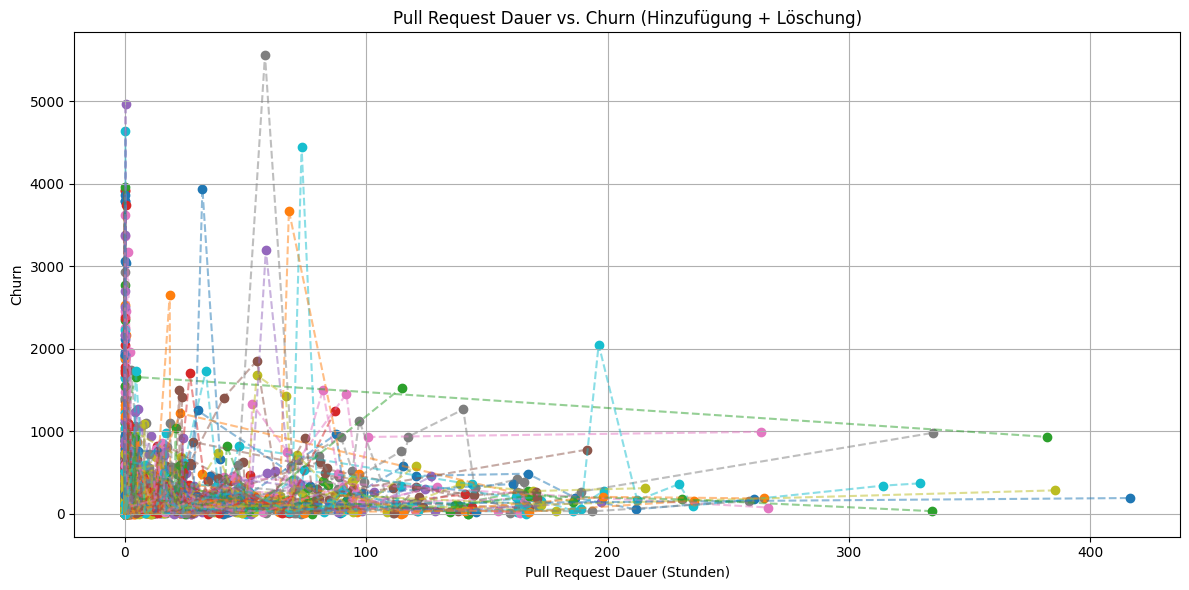
\includegraphics[width=\textwidth]{pr-latency-vs-churn-allgemein.png}
    \caption{Scatterplot der Churn-Werte in Relation zur PR-Latenz}
    \label{fig:pr-latency-vs-churn-allgemein}
\end{figure}

Dies wird ebenfalls durch die Berechnung des Spearman Rangkorrelationskoeffizienten deutlich, der bei einem Wert von 0.17 keine monotone Korrelation aufzeigt.

\subsection{Teilzeit vs. Vollzeit}
Die Auswertung der Daten ergibt, dass die Latency in den Vollzeitklassen mit 0.8 Stunden nahezu doppelt so hoch ist wie in den Teilzeitklassen, wo der Mittelwert bei 0.46 liegt. Bei den Churn-Werten ist hingegen kein signifikanter Unterschied erkennbar. Dies ist in der nachfolgenden \autoref{fig:vergleich-latency-churn} ersichtlich.

\begin{figure}[ht]
    \centering
    \begin{subfigure}[b]{0.48\textwidth}
        \centering
        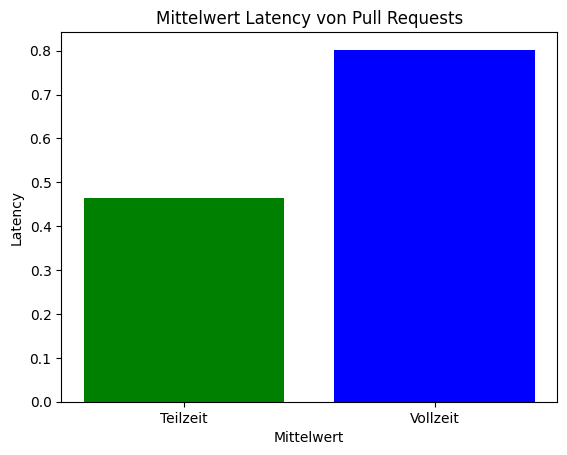
\includegraphics[width=\textwidth]{Figures/mittelwert-latency-t-v.png}
        \caption{Mittelwerte Latency Vollzeit vs. Teilzeit}
        \label{fig:mittelwert-latency-t-v}
    \end{subfigure}
    \hfill
    \begin{subfigure}[b]{0.48\textwidth}
        \centering
        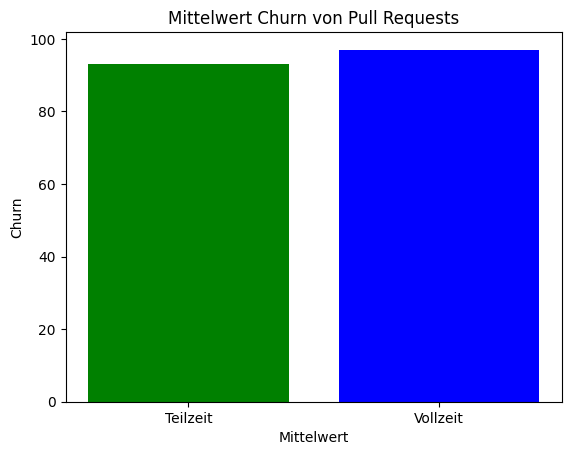
\includegraphics[width=\textwidth]{Figures/mittelwert-churn-t-v.png}
        \caption{Mittelwerte Churn Vollzeit vs. Teilzeit}
        \label{fig:mittelwert-churn-t-v}
    \end{subfigure}
    \caption{Vergleich von Latency und Churn zwischen Vollzeit und Teilzeit}
    \label{fig:vergleich-latency-churn}
\end{figure}

\newpage
Eine detaillierte Analyse der Latencies von Teilzeit- und Vollzeitstudierenden offenbart, dass Teilzeitklassen eine signifikant höhere Anzahl an Pull Requests aufweisen, die innerhalb einer Minute abgeschlossen werden. Dies zeigt sich im ersten Säulenpaar bei der \autoref{fig:anz-prs-vs-latency-tv}. Der Anteil der innerhalb einer Minute abgeschlossenen Pull Requests beläuft sich auf 16.8 Prozent der Gesamtzahl der Pull Requests bei den Teilzeitstudierenden, während dieser Anteil bei den Vollzeitstudierenden 9.9 Prozent beträgt. Bei allen Zeitabschnitten ausser 4–8 Stunden und 8–12 Stunden zeigen die Teilzeitklassen eine grössere Anzahl an Pull Requests, jedoch sind die grössten Differenzen bei den ersten drei und dem letzten Säulenpaar erkennbar. Eine Zusammenfassung der Pull Requests von 0 bis 30 Minuten ergibt, dass diese bei den Teilzeitklassen 50.7 Prozent und bei den Vollzeitklassen 44.7 Prozent ausmachen. Die letzte Säule zeigt einen Anteil von 18.6 Prozent für Teilzeitklassen und 19.7 Prozent für Vollzeitklassen. 
\begin{figure}[htbp]
    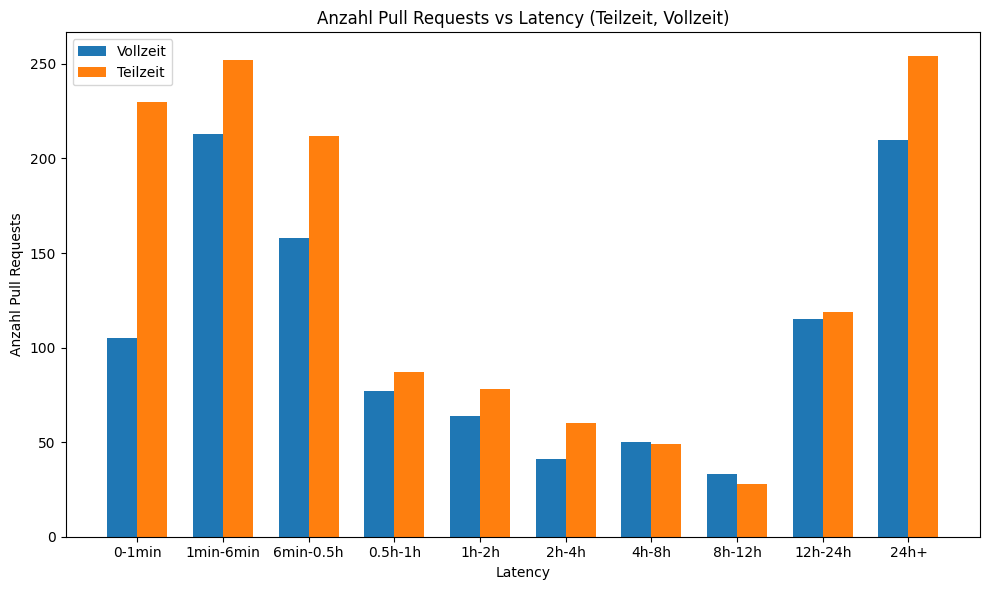
\includegraphics[width=\textwidth]{Figures/anz-prs-vs-latency-tv.png}
    \caption{Anzahl PullRequests vs. Latency (Teilzeit, Vollzeit)}
    \label{fig:anz-prs-vs-latency-tv}
\end{figure}

Die Entfernung der Datensätze, welche Merges zwischen Developer-Branches und Main-Branches abbilden, verändert die Resultate marginal. Dies ist in der \autoref{fig:anz-prs-vs-latency-tv-no-dev} ersichtlich. Ebenso überwiegen in den ersten drei Spaltenpaaren und im letzten Paar die Teilzeitklassen. Am auffälligsten ist wiederum das erste Säulenpaar. Hier beträgt der Anteil der Teilzeitstudierenden an der Gesamtzahl der Teilzeitstudierenden 16 Prozent und bei den Vollzeitklassen 9.3 Prozent. Die Anzahl der Pull-Requests, die in weniger als einer Minute bearbeitet werden, ist also in beiden Klassen zurückgegangen, liegt aber in beiden Fällen unter einem Prozent.
Addiert man die ersten drei Säulenpaare, so ergibt sich für die Teilzeitklassen ein Wert von 49.7 Prozent und für die Vollzeitklassen ein Wert von 43.3 Prozent. Damit liegen die Werte für die Teilzeit um genau ein Prozent und für die Vollzeit um 1.4 Prozent niedriger. Bei den 24 Stunden plus beträgt der Wert bei den Teilzeitklassen 19 Prozent, was einer Differenz von 0.4 Prozent entspricht. Bei den Vollzeitklassen beträgt der Wert 20.2 Prozent, was einem Anstieg von 0.5 Prozent gleichkommt.

\begin{figure}[htbp]
    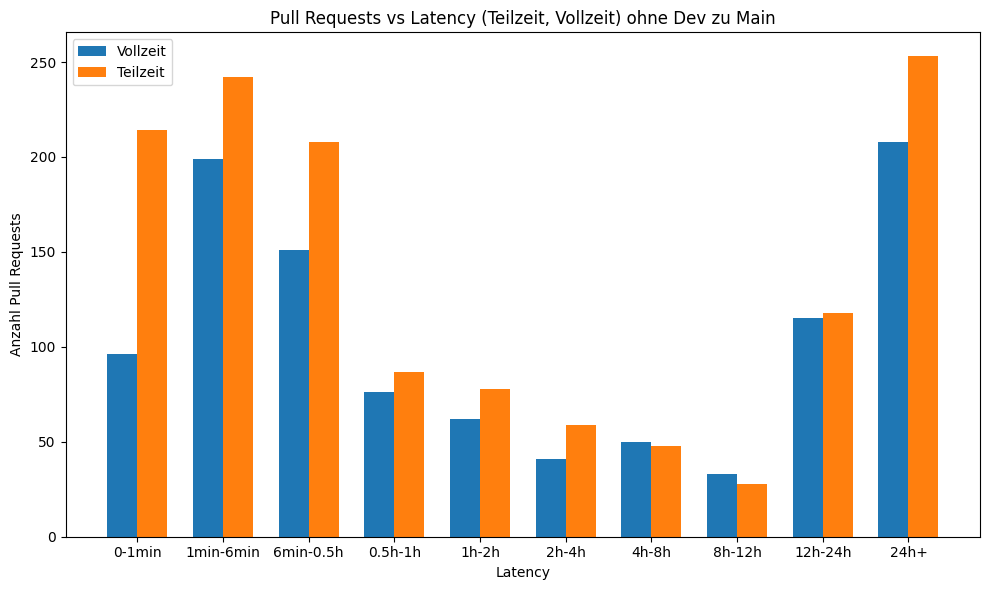
\includegraphics[width=\textwidth]{Figures/anz-prs-vs-latency-tv-no-dev.png}
    \caption{Anzahl PullRequests vs. Latency (Teilzeit, Vollzeit) ohne Dev zu Main}
    \label{fig:anz-prs-vs-latency-tv-no-dev}
\end{figure}

\newpage
\subsection{Ergebnisse Einfluss Projektzeit}
Anhand der \autoref{fig:mittelwert-woche-lateny} ist ersichtlich, dass die Latency gegen Ende der Projektzeit abnimmt. Während die Churn (\autoref{fig:mittelwert-woche-churn}) bis zur 5. Woche ansteigt. 
Zu beachten ist, dass, wie bereits im Kapitel \secref{sec:Projektmodule} erwähnt, die Projekte nicht exakt 28 Tage dauern. Die ermittelten Projektlaufzeiten liegen zwischen 20 und 36 Tagen.
Wobei die Klassen aus den Jahren 2021 und 2022 bei einem Durchschnitt von 21 Tagen liegen. Die neueren Klassen ab dem Jahr 2023 haben eine Projektlaufzeitspannweite von 28 bis 36 Tagen. Wovon eine Klasse die 35 Tage überschreitet. In dieser Klasse haben fünf Teams eine Laufzeit von 29 Tagen und drei Teams eine Laufzeit von 35 oder 36 Tagen. Somit widerspiegeln diese drei Teams die Woche sechs in der folgenden \autoref{fig:vergleich-latency-churn-projektzeit}. Die Latency nimmt im Laufe der Zeit zweimal stark ab. Das erste Mal von der ersten zur zweiten Projektwoche, wobei sie in der ersten Woche bei einem Mittelwert von 3.5 Stunden und in der zweiten Woche bei 2 Stunden liegt. Zum zweiten Mal nimmt die Latenz in der vierten Projektwoche stark ab, und zwar von 1.7 Stunden auf 0.5 Stunden. In der sechsten Woche ist die Latency nahezu 0. Der Churn steigt bis zur 5. Woche kontinuierlich von 72 Zeilenwechseln auf 115 an und sinkt dann in der 6. Woche auf 98.
\begin{figure}[htbp]
    \centering
    \begin{subfigure}[b]{0.48\textwidth}
        \centering
        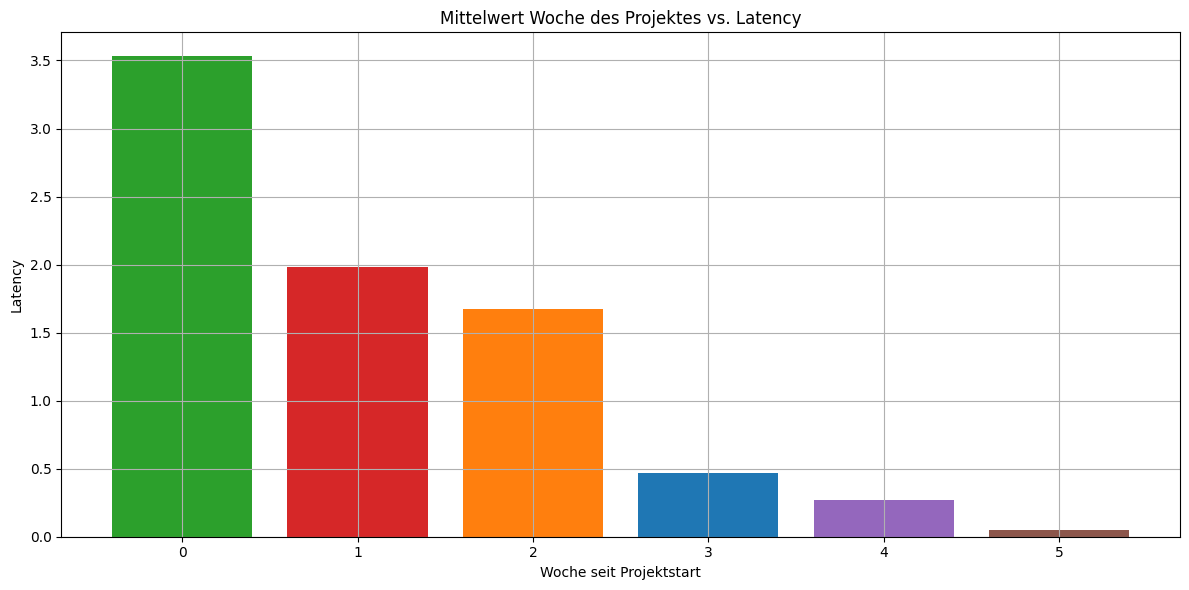
\includegraphics[width=\textwidth]{Figures/mittelwert-woche-lateny.png}
        \caption{Mittelwerte Woche des Projektes vs. Latency}
        \label{fig:mittelwert-woche-lateny}
    \end{subfigure}
    \hfill
    \begin{subfigure}[b]{0.48\textwidth}
        \centering
        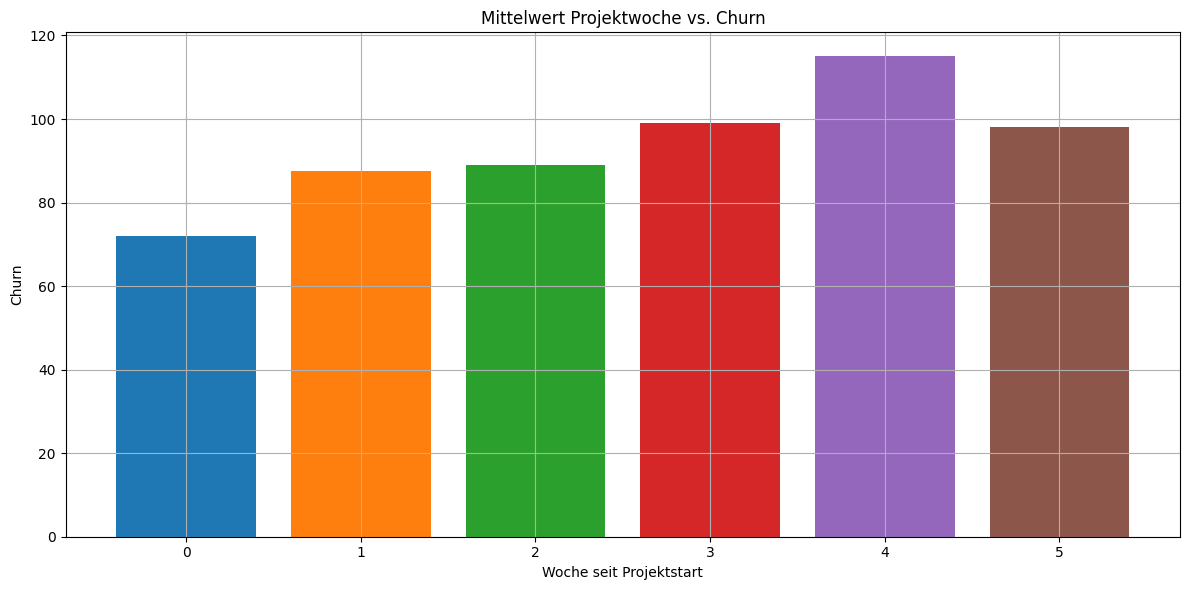
\includegraphics[width=\textwidth]{Figures/mittelwert-woche-churn.png}
        \caption{Mittelwerte Woche des Projektes vs. Churn}
        \label{fig:mittelwert-woche-churn}
    \end{subfigure}
    \caption{Vergleich von Latency und Churn innerhalb der Projektzeit}
    \label{fig:vergleich-latency-churn-projektzeit}
\end{figure}

Werden die Daten nach Vollzeit- und Teilzeitstudierenden aufgeteilt, zeigt sich bei den Vollzeitklassen ein ähnliches Bild. Veranschaulicht wird dies in der \autoref{fig:vergleich-latency-churn-projektzeit-v}. Allerdings ist der Mittelwert der Latecy in der ersten Woche mit 7.4 Stunden mehr als doppelt so hoch wie in der Gesamtauswertung. Ebenso nimmt die Latency von der ersten zur zweiten Woche stark ab. Der Wert sinkt um mehr als die Hälfte und liegt anschliessend bei 3.4 Stunden. Ab der vierten Woche ist der Mittelwert unter einer halben Stunde. Zeitgleich ist der Churn in der ersten Woche mit 71 Zeilenänderungen am geringsten, steigt mit Ausnahme der dritten Woche an und erreicht in der fünften Woche mit 121 Änderungen seinen Höhepunkt. Im Gegensatz zur Latency liegen diese Werte sehr nahe bei der Gesamtanalyse.
\begin{figure}[htbp]
    \centering
    \begin{subfigure}[b]{0.48\textwidth}
        \centering
        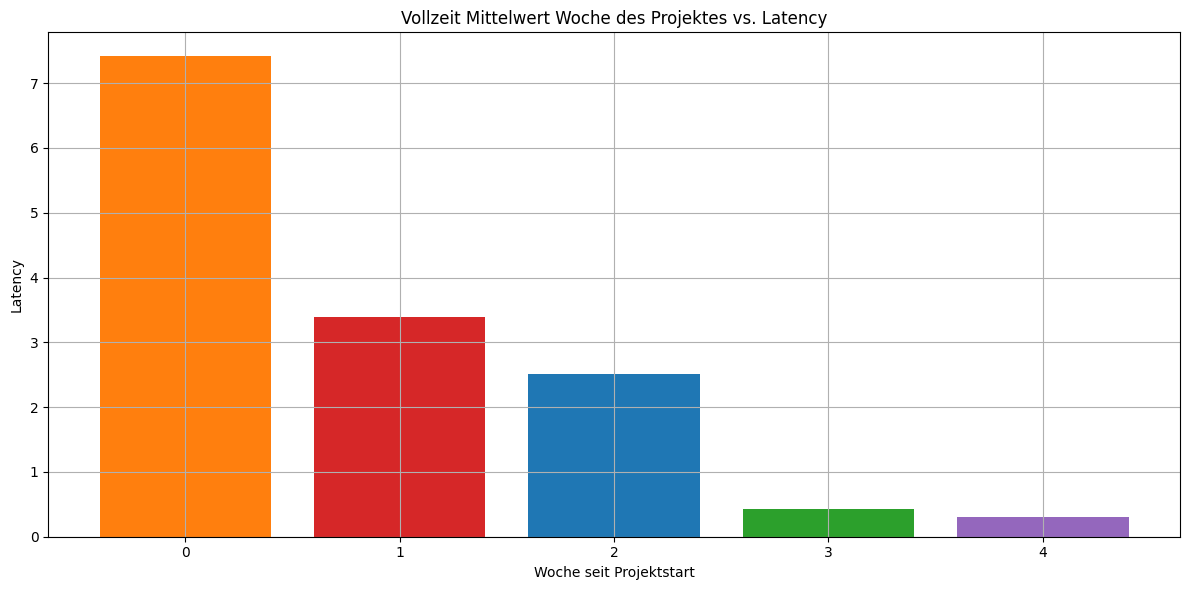
\includegraphics[width=\textwidth]{Figures/mittelwert-woche-lateny-v.png}
        \caption{Mittelwerte Woche des Projektes vs. Latency Vollzeit}
        \label{fig:mittelwert-woche-lateny-v}
    \end{subfigure}
    \hfill
    \begin{subfigure}[b]{0.48\textwidth}
        \centering
        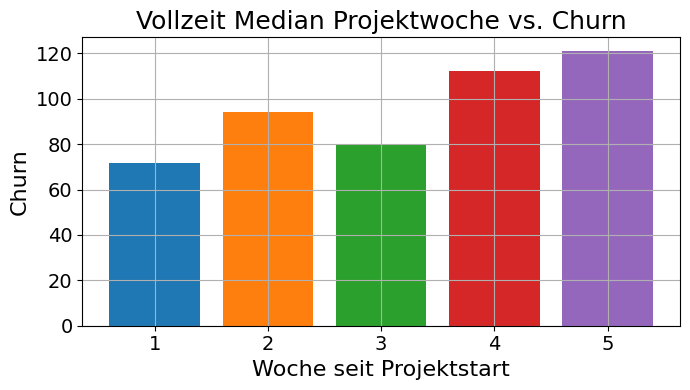
\includegraphics[width=\textwidth]{Figures/mittelwert-woche-churn-v.png}
        \caption{Mittelwerte Woche des Projektes vs. Churn Vollzeit}
        \label{fig:mittelwert-woche-churn-v}
    \end{subfigure}
    \caption{Vergleich von Latency und Churn innerhalb der Projektzeit Vollzeit}
    \label{fig:vergleich-latency-churn-projektzeit-v}
\end{figure}

In der \autoref{fig:vergleich-latency-churn-projektzeit-t} ist zu erkennen, dass auch bei den Teilzeitstudierenden die Latency in der ersten Woche am höchsten ist, sich aber weniger stark von den Wochen zwei und drei unterscheidet. Zusätzlich ist der Wert der ersten Woche im Gegensatz zur Gesamtanalyse und vor allem den Vollzeitstudierenden tiefer bei einem Wert von knapp 2 Stunden. Zudem steigt bei den Teilzeitklassen in der dritten Woche die Latency nochmals an, aber dies nur mit einem Unterschied von 0.1 Stunden. Danach sinkt die Latency ebenso und liegt in Woche vier unter einer Stunde. Der Churn steigt ebenfalls an und erreicht in Woche fünf seinen Höhepunkt bei 110 Codezeilenänderungen. Die Werte der Churn befinden sich im gleichen Rahmen wie bei den Vollzeitstudierenden.

\begin{figure}[htbp]
    \centering
    \begin{subfigure}[b]{0.48\textwidth}
        \centering
        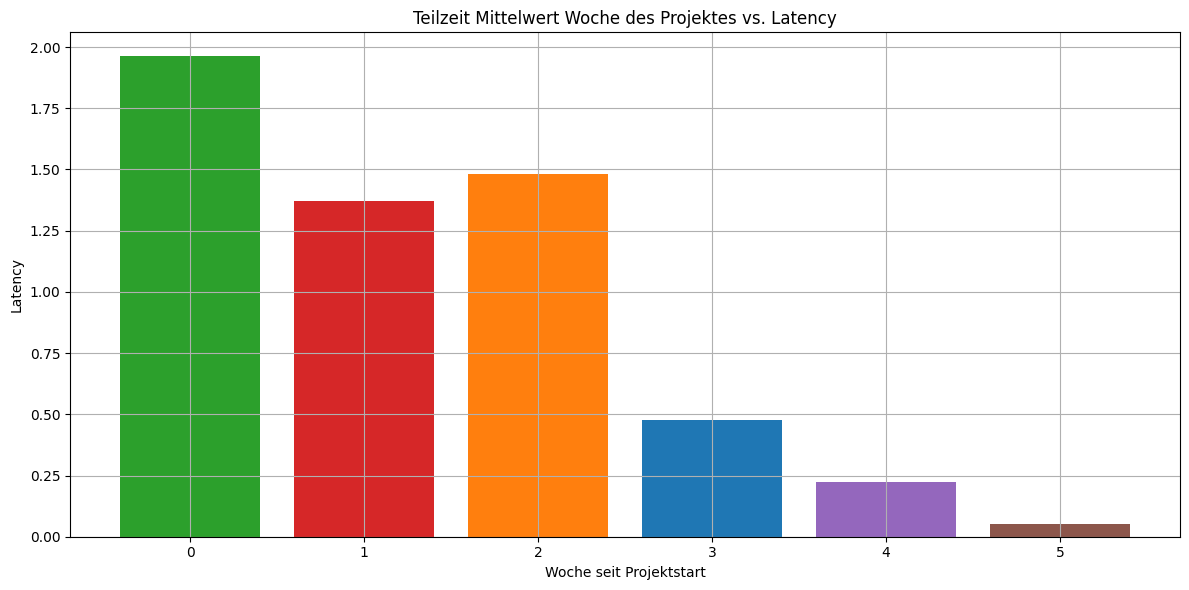
\includegraphics[width=\textwidth]{Figures/mittelwert-woche-lateny-t.png}
        \caption{Mittelwerte Woche des Projektes vs. Latency Teilzeit}
        \label{fig:mittelwert-woche-lateny-t}
    \end{subfigure}
    \hfill
    \begin{subfigure}[b]{0.48\textwidth}
        \centering
        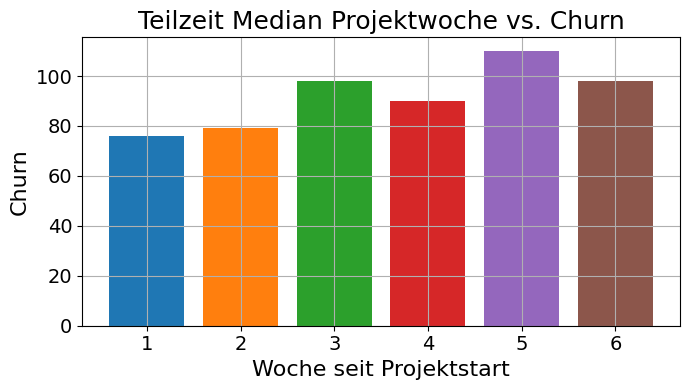
\includegraphics[width=\textwidth]{Figures/mittelwert-woche-churn-t.png}
        \caption{Mittelwerte Woche des Projektes vs. Churn Teilzeit}
        \label{fig:mittelwert-woche-churn-t}
    \end{subfigure}
    \caption{Vergleich von Latency und Churn innerhalb der Projektzeit Teilzeit}
    \label{fig:vergleich-latency-churn-projektzeit-t}
\end{figure}

\newpage
Die Analyse der Daten, die in der \autoref{fig:anz-prs-vs-latency-tv} dargestellt sind, zeigt, dass eine Vielzahl von PullRequests innerhalb einer halben Stunde bearbeitet wurde. Eine detaillierte Analyse dieser kurz geöffneten PullRequests offenbart, dass der überwiegende Teil davon in den letzten drei Tagen und insbesondere am Tag der Abgabe erstellt wurde. Eine weitere Restriktion der Pull Requests auf jene, die innerhalb einer Minute abgearbeitet wurden, resultiert in einer ähnlichen Situation. Es ist jedoch festzustellen, dass der Tag der Abgabe sich stärker abhebt, wobei auch ein Anstieg zwei Tage vor Abgabe zu erkennen ist.  Die Resultate sind in \autoref{fig:anz-prs-under-x-mins} dargestellt.

\begin{figure}[htbp]
    \centering
    \begin{subfigure}[b]{0.48\textwidth}
        \centering
        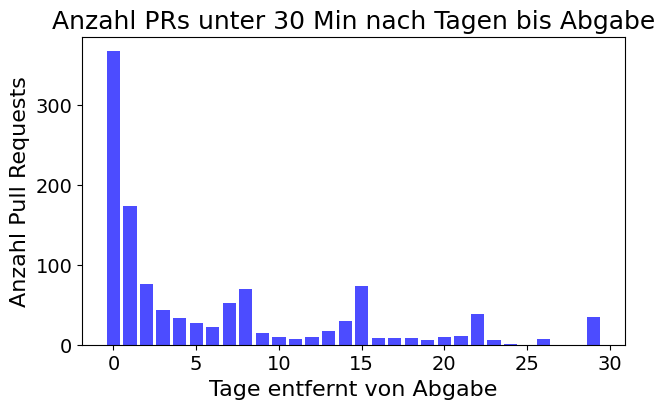
\includegraphics[width=\textwidth]{Figures/anz-prs-under-30-min.png}
    \caption{Anzahl PullRequests unter 30 Minuten im Verhältnis zur Abgabe}
    \label{fig:anz-prs-under-30-min}
    \end{subfigure}
    \hfill
    \begin{subfigure}[b]{0.48\textwidth}
        \centering
        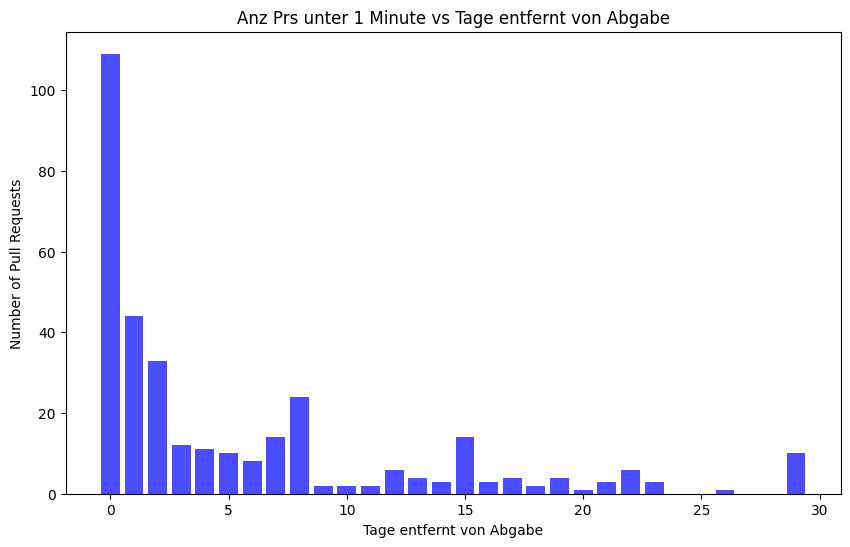
\includegraphics[width=\textwidth]{Figures/anz-prs-under-1-min.png}
    \caption{Anzahl PullRequests unter einer Minute im Verhältnis zur Abgabe}
    \label{fig:anz-prs-under-1-min}
    \end{subfigure}
    \caption{Anzahl PullRequests unter 30 / 1 Minute im Verhältnis zur Abgabe}
    \label{fig:anz-prs-under-x-mins}
\end{figure}

Die Untersuchung von Pull Requests im Verhältnis zur Abgabe zeigt, dass am Tag der Abgabe die meisten Pull Requests abgearbeitet wurden. Dies ist aus der \autoref{fig:anz-prs-days-away-from-end} ersichtlich. Von den 2427 untersuchten Pull Requests wurden 523 am Tag der Abgabe erstellt und abgeschlossen. Dieser Wert entspricht einer Quote von 21.5 Prozent.  Die zweitmeisten Pull Request wurden am Tag vor der Abgabe bearbeitet mit einer Anzahl von 309. Am drittletzten Tag wurde ein erhöhter Wert festgestellt, der jedoch nicht mehr signifikant hervorsticht. Es wurden 154 Pull Requests bearbeitet. Eine Zusammenfassung der letzten drei Tage der Projekte ergibt eine Gesamtzahl von 986 bearbeiteten Pull Requests, was einem Prozentsatz von 40.6 Prozent entspricht. Über die restliche Projektzeit variieren die Anzahl bearbeiteten Pull Rquests. Es lassen sich erhöhte Werte sieben, acht und 15 Tage vor der Abgabe feststellen, die sich von den Werten der übrigen Tage abheben.
\begin{figure}[htbp]
    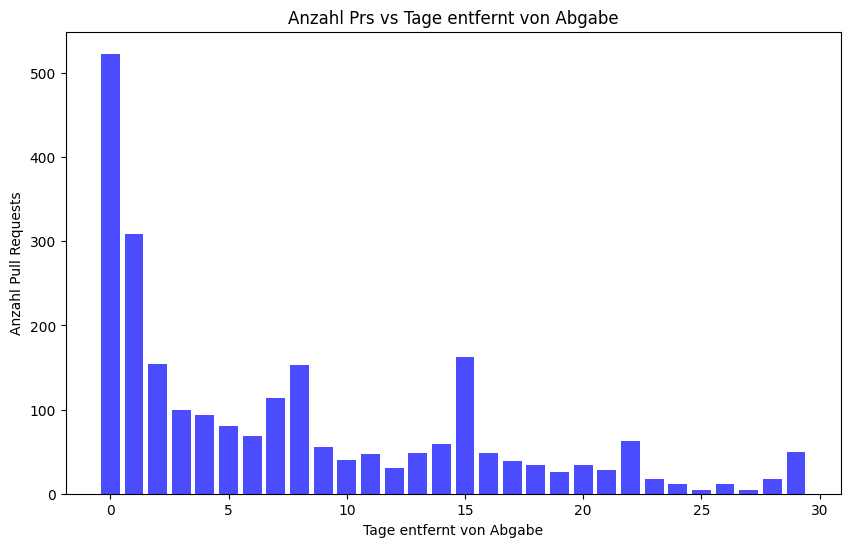
\includegraphics[width=\textwidth]{Figures/anz-prs-days-away-from-end.png}
    \caption{Anzahl geschlossene Pull Requests im Verhältnis zur Abgabe}
    \label{fig:anz-prs-days-away-from-end}
\end{figure}
\newpage
Eine detaillierte Analyse der Pull Requests in den einzelnen Teams zeigt, dass in 19 von 71 Teams mehr als 50 Prozent aller Pull Requests in den letzten drei Projekttagen eröffnet und abgeschlossen wurden. Es lässt sich feststellen, dass vier der analysierten Teams einen Anteil von über 75 Prozent ihrer Pull Requests in diesem Zeitraum bearbeitet haben. Zudem ist eine Gruppe zu identifizieren, die sämtliche ihrer Pull Requests innerhalb des definierten Zeitraums erstellt und geschlossen hat. Eine detaillierte Analyse des Projektes ergab, dass die genannte Gruppe insgesamt zwei Pull Requests hatte, die beide am Tag vor der Abgabe erstellt wurden. Wenn diese Analyse auf den letzten Projekttag beschränkt wird, dann sind es drei Teams, die mehr als 50 Prozent ihrer Pull Requests am Abgabetag erledigt haben.

\section{Ergebnisse Pull Reqeust Akzeptanz}
Für die Analyse der geschlossenen Pull Requests (PRs) wurden zunächst alle verfügbaren PRs eingelesen und entsprechend gefiltert. Erste Auswertungen ergaben, dass lediglich 0,07\% aller Pull Requests geschlossen wurden. Von den insgesamt 170 geschlossenen PRs entfallen 95 auf die Vollzeitklassen und 75 auf die Teilzeitklassen, obwohl der analysierte Datenbestand 27 Vollzeitprojekte und 43 Teilzeitprojekte umfasst. Der durchschnittliche Churn der PRs liegt in den Teilzeitklassen ebenfalls niedriger (137 im Vergleich zu 188 bei den Vollzeitklassen).

Abbildung \autoref{fig:anz-clsd-prs-nach-churn} zeigt die Anzahl geschlossener PRs, gruppiert nach ihrer Churn-Grösse. Dabei wird deutlich, dass in den Teilzeitklassen vor allem kleinere PRs abgelehnt wurden. Eine manuelle Analyse der Gründe für das Scheitern dieser PRs ergab, dass viele ohne jeglichen Kommentar abgelehnt wurden. Ob dies daran lag, dass die Implementierung nicht mehr benötigt wurde oder fehlerhaft war, lässt sich im Nachhinein nicht eindeutig klären.

\begin{figure}[htbp]
    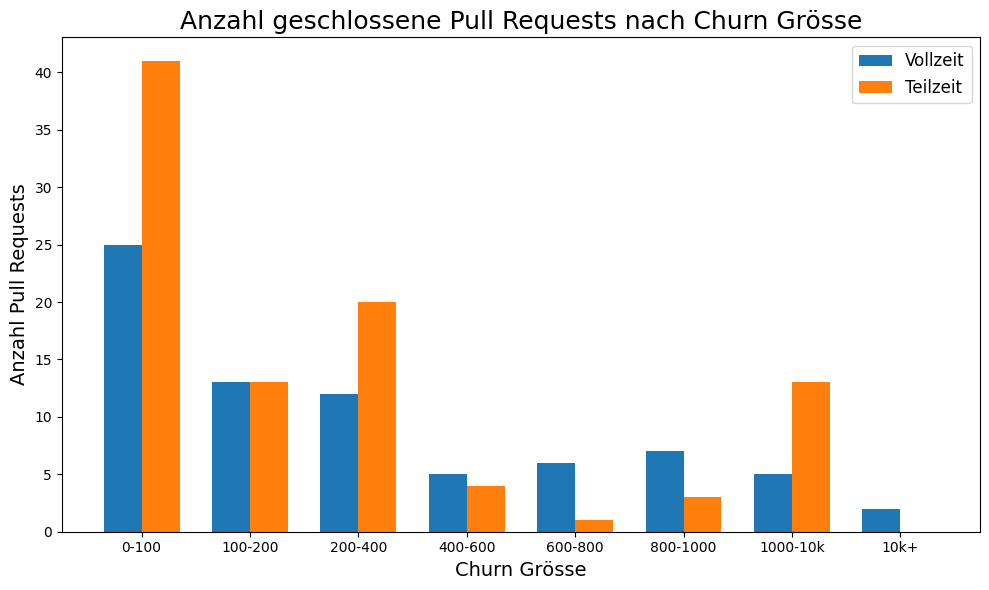
\includegraphics[width=\textwidth]{Figures/anzahl-geschlossene-prs-nach-churn.png}
    \caption{Anzahl geschlossene Pull Requests nach Churn Grösse}
    \label{fig:anz-clsd-prs-nach-churn}
\end{figure}


Die manuelle Analyse der geschlossenen PRs mit einem Churn von über 500 zeigte hingegen ein anderes Bild: Diese PRs wurden häufig aufgrund eines falschen Zielbranches erstellt. In mehreren Fällen konnte ausserdem beobachtet werden, dass das vorgeschlagene Feature bereits durch einen anderen Branch implementiert worden war. Gewisse PRs wurden auch für grosse Refactoring Arbeiten verwendet. 

Die Kategorie 'divers' beinhaltet hauptsächlich Feedback-PRs, welche von gewissen Dozenten für die Notenvergabe verwendet wurden. Ausserdem sind einige refactor Branches zu sehen, welche Ausschliesslich für den Refactoren erstellt wurden und anschliessend geschlossen wurden. 

\begin{table}
\caption{Geschlossene PRs gruppiert nach Ursache}
\label{tab:treatments}
\centering
\begin{tabular}{l l l l l l l}
\toprule
\textbf{Klasse} & 
\makecell{\textbf{PR abgelehnt} \\ \textbf{ohne Grund}} & 
\makecell{\textbf{Feat. durch} \\ \textbf{anderen PR impl.}} & 
\makecell{\textbf{Feat. nicht} \\ \textbf{mehr benötigt}} & 
\makecell{\textbf{Impl.} \\ \textbf{abgelehnt}} & 
\makecell{\textbf{falscher} \\ \textbf{Zielbranch}} &
\makecell{\textbf{divers}} \\
\midrule
T < 100& 35 & 1 & 3 & 2 & 0 & 0\\
V < 100& 22 & 1 & 0 & 1 & 1 & 0 \\
T > 500& 22 & 8 & 0 & 2 & 4 & 5 \\
V > 500& 8 & 0 & 1 & 4 & 6 & 0 \\
\bottomrule
\end{tabular}
\end{table}
\newpage
\noindent\textbf{Legende:}
\begin{itemize}
\item[$T$] Alle Teilzeitklassen
\item[$V$] Alle Vollzeitklassen
\item[$< 100$] Churn kleiner 100
\item[$> 500$] Churn größer 500
\end{itemize}

\subsection{Ergebnisse Einfluss Projektzeit}
Wie in Abbildung \autoref{fig:closed-prs-projektkeit-teilzeit} deutlich wird, wurden die meisten Pull Requests (PRs) in den Teilzeitklassen am letzten Tag vor der Projektabgabe geschlossen. Dieser Effekt ist zwar auch in den Vollzeitklassen erkennbar, jedoch weniger ausgeprägt. In Abbildung \autoref{fig:closed-prs-projektkeit-vollzeit} wird zudem deutlich, dass die geschlossenen PRs in den Vollzeitklassen gleichmässiger über den gesamten Projektzeitraum verteilt sind.

\begin{figure}[htbp]
    \centering
    \begin{subfigure}[b]{0.48\textwidth}
        \centering
        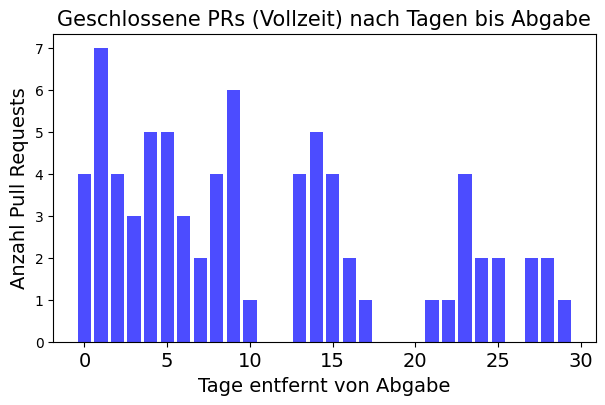
\includegraphics[width=\textwidth]{Figures/closed-prs-projektzeit-vollzeit.png}
        \caption{Anzahl geschlossene PRs Vollzeitklassen nach Tagen entfernt von Abgabe}
        \label{fig:closed-prs-projektkeit-vollzeit}
    \end{subfigure}
    \hfill
    \begin{subfigure}[b]{0.48\textwidth}
        \centering
        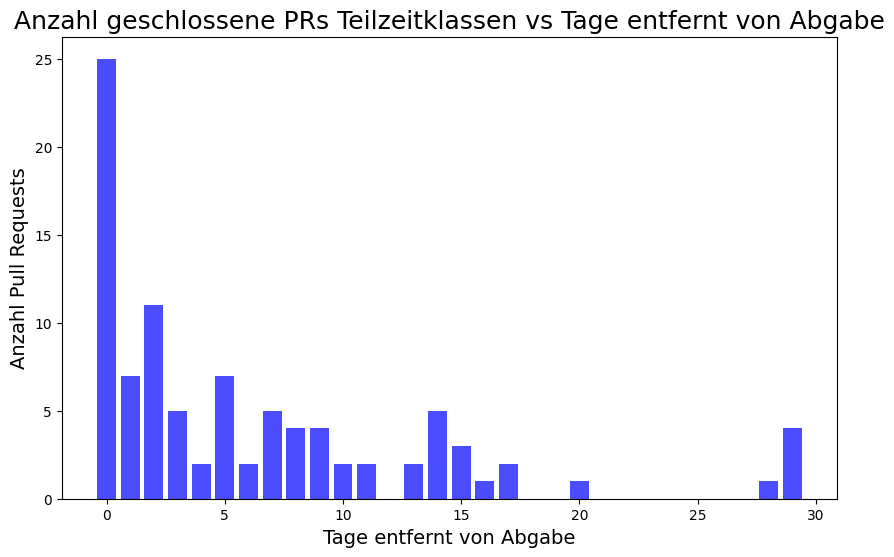
\includegraphics[width=\textwidth]{Figures/closed-prs-projektzeit-teilzeit.png}
         \caption{Anzahl geschlossene PRs Teilzeitklassen nach Tagen entfernt von Abgabe}
        \label{fig:closed-prs-projektkeit-teilzeit}
    \end{subfigure}
    \caption{Vergleich Anzahl geschlossene PRs Teilzeit vs Vollzeit nach Tagen entfernt von Abgabe}
    \label{fig:vergleich-latency-churn-projektzeit}
\end{figure}


\section{Ergebnisse Entwicklungsaktivität}
Empirische Studien zeigen, dass die Entwicklungsaktivität in Open-Source-Projekten auf Plattformen wie GitHub charakteristische Muster im Wochenverlauf aufweist. Insbesondere an Wochenenden ist die Aktivität signifikant geringer als unter der Woche. Innerhalb der Arbeitswoche fallen Montag und Freitag häufig als die Tage mit der geringsten Aktivität auf. Das Phänomen des Rückgangs der Entwicklungsaktivität wird oftmals auch \textit{Friday Effect} genannt. \parencite{claes_programmers_2018}

Da sich während der Analyse deutliche Differenzen zwischen den Voll- und Teilzeitklassen ergaben, wurden diese in der Analyse geteilt angeschaut. 

Auch in den vorliegenden Daten zeigt sich eine Tendenz zur Konzentration der Aktivitäten auf spezifische Wochentage, insbesondere auf die jeweiligen Unterrichtstage. So wurden bei den Vollzeitklassen rund 24\,\% aller Pull Requests (PRs) am Projekttag erstellt. Bei den Teilzeitklassen liegt dieser Wert mit 34\,\% deutlich höher. Dies unterstreicht die Bedeutung des Unterrichtstages für die praktische Arbeit im Rahmen des Projekts.

Abbildung \autoref{fig:anz-prs-teilzeit-pro-wochentag} zeigt exemplarisch die Verteilung der PR-Erstellungen über die Wochentage für zwei Teilzeitklassen. Deutlich erkennbar ist ein Aktivitätspeak am jeweiligen Unterrichtstag. An den darauffolgenden Tagen nimmt die Aktivität deutlich ab. Auffällig ist zudem, dass PRs nicht nur am Unterrichtstag erstellt, sondern auch überprüft und geschlossen wurden. Insgesamt wurden 27.7\,\% aller PRs der Teilzeitklassen am Wochenende erstellt – ein vergleichsweise hoher Wert.

\begin{figure}[htbp]
    \centering
    \begin{subfigure}[b]{0.48\textwidth}
        \centering
        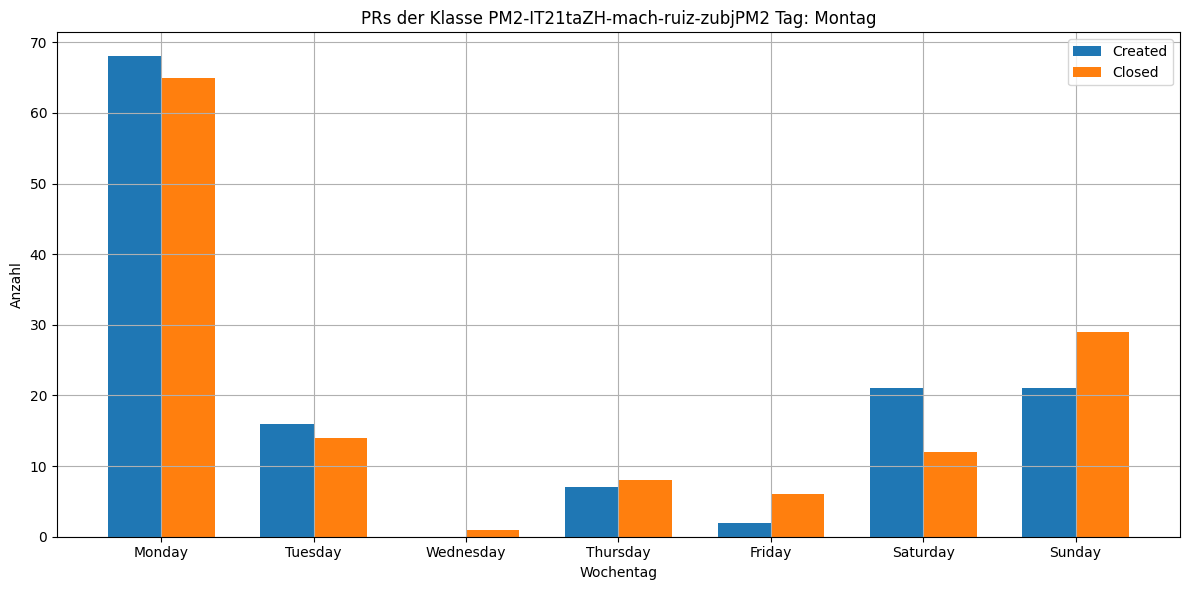
\includegraphics[width=\textwidth]{Figures/pr-klasse-per-wochentag-it21ta.png}
         \caption{Anzahl geöffneter PRs pro Wochentag der Teilzeitklasse It21ta}
        \label{fig:anzahl-prs-pro-wochentag-it21ta}
    \end{subfigure}
    \hfill
    \begin{subfigure}[b]{0.48\textwidth}
        \centering
        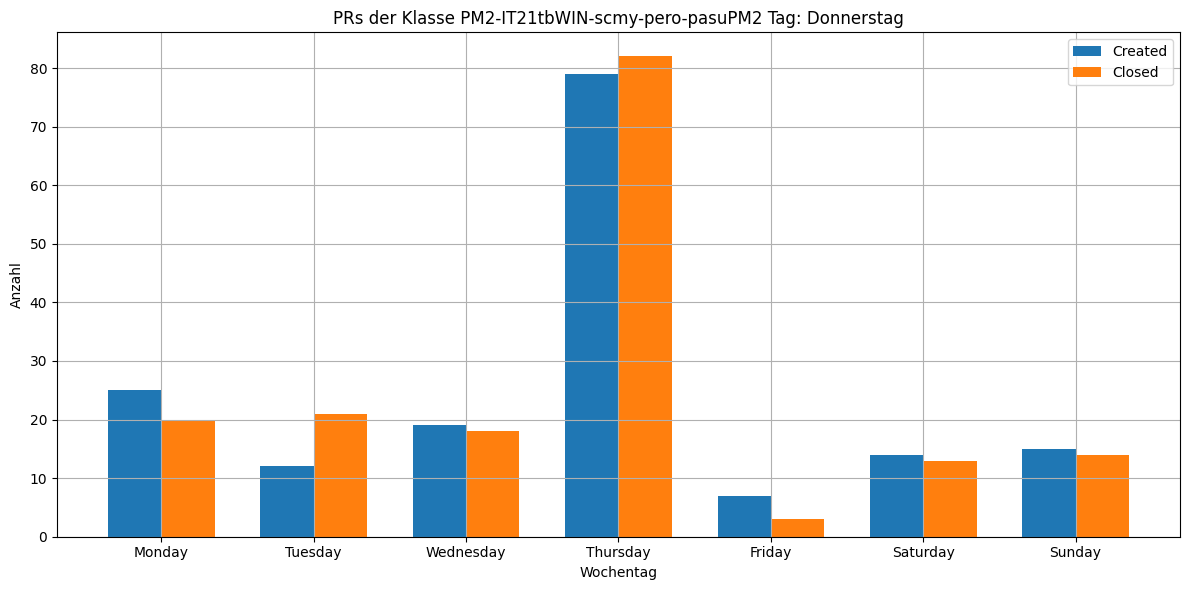
\includegraphics[width=\textwidth]{Figures/pr-klasse-per-wochentag-21tb.png}
         \caption{Anzahl geöffneter PRs pro Wochentag der Teilzeitklasse It21tb}
        \label{fig:anzahl-prs-pro-wochentag-it21tb}
    \end{subfigure}
    \caption{Anzahl geöffneter PRs pro Wochentag von 2 Teilzeitklassen}
    \label{fig:anz-prs-teilzeit-pro-wochentag}
\end{figure}

Ein kontrastierendes Bild zeigt sich bei den Vollzeitklassen. Abbildung \autoref{fig:anz-prs-vollzeit-pro-wochentag} zeigt die Verteilung der PR-Erstellungen bei zwei exemplarischen Klassen. 
Hier zeigt sich eine insgesamt gleichmässigere Verteilung der Aktivitäten über die Woche. Zwar ist auch hier der Projekttag der aktivste, jedoch in geringerem Ausmass als bei den Teilzeitklassen. Zudem wurden nur 16.8\% der PRs am Wochenende erstellt.

\begin{figure}[htbp]
    \centering
    \begin{subfigure}[b]{0.48\textwidth}
        \centering
        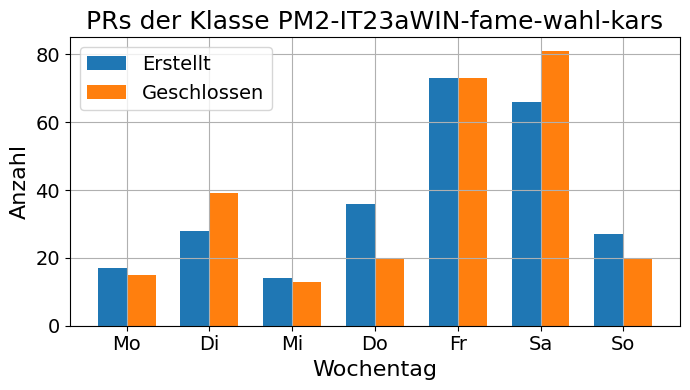
\includegraphics[width=\textwidth]{Figures/pr-klasse-per-wochentag-23a.png}
         \caption{Anzahl geöffneter PRs pro Wochentag der Vollzeitklasse It23a}
        \label{fig:anzahl-prs-pro-wochentag-it23a}
    \end{subfigure}
    \hfill
    \begin{subfigure}[b]{0.48\textwidth}
        \centering
        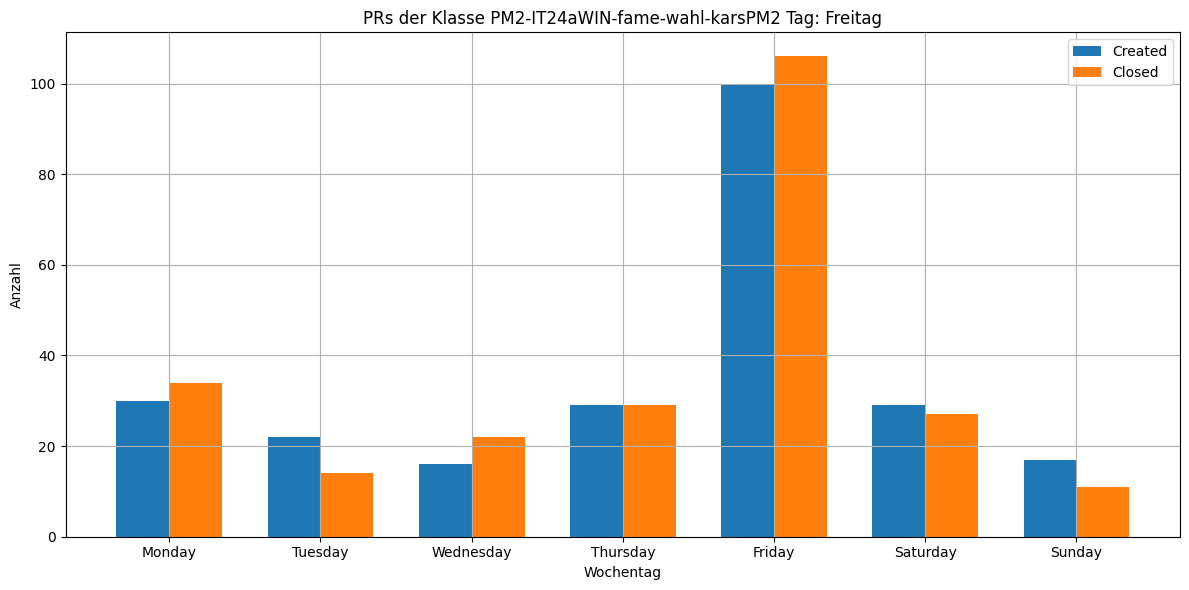
\includegraphics[width=\textwidth]{Figures/pr-klasse-per-wochentag-24a.png}
         \caption{Anzahl geöffneter PRs pro Wochentag der Vollzeitklasse It24a}
        \label{fig:anzahl-prs-pro-wochentag-it24a}
    \end{subfigure}
    \caption{Anzahl geöffneter PRs pro Wochentag von 2 Vollzeitklassen}
    \label{fig:anz-prs-vollzeit-pro-wochentag}
\end{figure}

\subsection{Ereignisse Analyse Commits}
Da nicht nur die PRs sondern auch die einzelnen Commits interessant für die Entwicklungsanalyse ist, wurden die Commits der PRs angeschaut. 
Die Analyse bestätigte die Resultate, welche in der PR Analyse bereits schon gefunden wurden. 

So wurden bei den Vollzeitklassen 23.7\,\% aller Commits am jeweiligen Unterrichtstag durchgeführt. Bei den Teilzeitklassen liegt dieser Anteil mit 33.9\,\% deutlich höher. Abbildung \autoref{fig:anz-commits-teilzeit-pro-wochentag} zeigt die Verteilung der Commits über die Wochentage exemplarisch für zwei Teilzeitklassen. Erkennbar ist – analog zur PR-Verteilung – ein deutlicher Peak an den jeweiligen Projekttagen. Insgesamt wurden 25.9\,\% aller Commits der Teilzeitklassen an einem Samstag oder Sonntag durchgeführt.

\begin{figure}[htbp]
    \centering
    \begin{subfigure}[b]{0.48\textwidth}
        \centering
        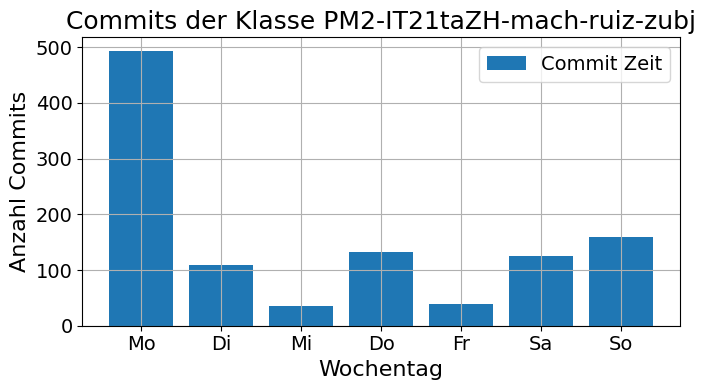
\includegraphics[width=\textwidth]{Figures/commits-klasse-per-wochentag-21ta.png}
         \caption{Anzahl Commits pro Wochentag der Teilzeitklasse It21ta}
        \label{fig:anzahl-commits-pro-wochentag-it21ta}
    \end{subfigure}
    \hfill
    \begin{subfigure}[b]{0.48\textwidth}
        \centering
        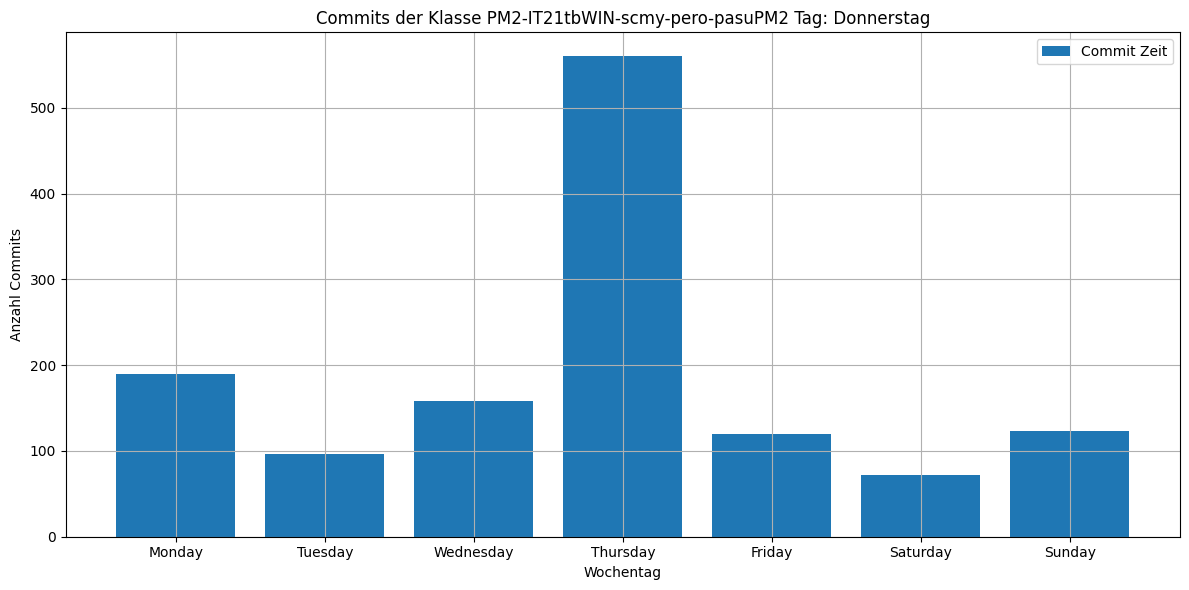
\includegraphics[width=\textwidth]{Figures/commits-klasse-per-wochentag-21tb.png}
         \caption{Anzahl Commits pro Wochentag der Teilzeitklasse It21tb}
        \label{fig:anzahl-commits-pro-wochentag-it21tb}
    \end{subfigure}
    \caption{Anzahl Commits pro Wochentag von 2 Teilzeitklassen}
    \label{fig:anz-commits-teilzeit-pro-wochentag}
\end{figure}

Ein ähnliches Bild ergibt sich bei den Vollzeitklassen. Abbildung \autoref{fig:anz-commits-vollzeit-pro-wochentag} zeigt die Commits zweier exemplarischer Klassen. Hier wurden 23.7\,\% der Commits am jeweiligen Projekttag durchgeführt – identisch mit dem PR-Anteil. Am Wochenende hingegen wurden nur 19.4\,\% der Commits verzeichnet, was deutlich unter dem Wert der Teilzeitklassen liegt.

\begin{figure}[htbp]
    \centering
    \begin{subfigure}[b]{0.48\textwidth}
        \centering
        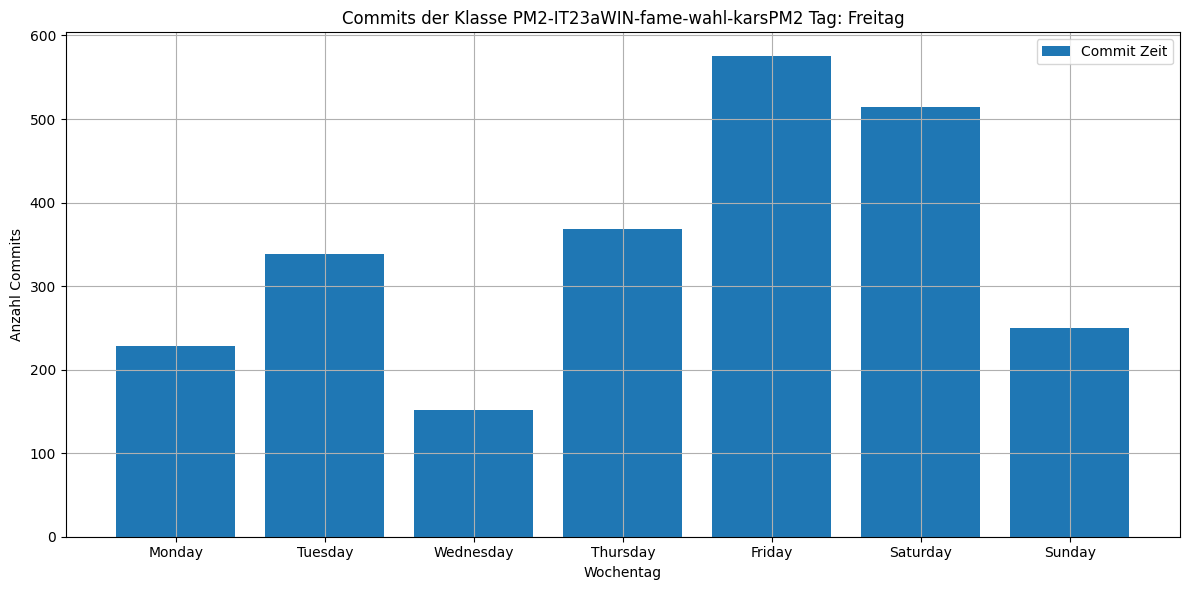
\includegraphics[width=\textwidth]{Figures/commits-klasse-per-wochentag-23a.png}
         \caption{Anzahl Commits pro Wochentag der Teilzeitklasse It23a}
        \label{fig:anzahl-commits-pro-wochentag-it23a}
    \end{subfigure}
    \hfill
    \begin{subfigure}[b]{0.48\textwidth}
        \centering
        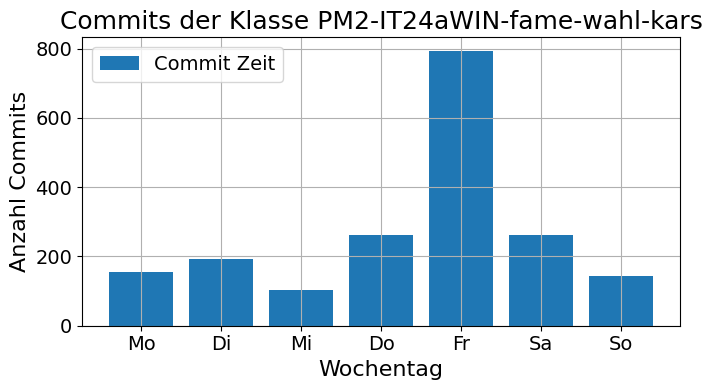
\includegraphics[width=\textwidth]{Figures/commits-klasse-per-wochentag-24a.png}
         \caption{Anzahl Commits pro Wochentag der Teilzeitklasse It24a}
        \label{fig:anzahl-commits-pro-wochentag-it24a}
    \end{subfigure}
    \caption{Anzahl Commits pro Wochentag von 2 Vollzeitklassen}
    \label{fig:anz-commits-vollzeit-pro-wochentag}
\end{figure}

\section{Projektmodul Ergebnisse bei Open Source Projekten}
\subsection{Latency und Churn}
\subsection{Allgemeine Korrelationen}
